% Jonathan Forhan
% EG-340 Project 1

\documentclass[12pt]{article}

\title{EE-340 Project 1}
\author{Jonathan Forhan\\ EE340\\ Southern New Hampshire University\\ Spring 2024}
\date{ }

\usepackage{geometry}
\usepackage{amsmath}
\usepackage[none]{hyphenat}
\usepackage{graphicx}

\renewcommand{\thesubsection}{\thesection-\alph{subsection}}

\begin{document}

\maketitle
\thispagestyle{empty}
\clearpage

\section{Problem statement}

In many scientific and engineering disciplines, understanding the distribution of
sample means and variances is crucial for making informed decisions and drawing
accurate conclusions. The probability density functions (PDFs) of these statistical
parameters provide valuable insights into the variability and reliability of experimental
data. \\ \\
This project aims to visualize the probability density functions of sample means and variances.

\section{Results}

\[
	\begin{aligned}
		\textrm{let } & \mu_x        =2 \\
		\textrm{let } & \mu_y        =1 \\
		\textrm{let } & \sigma_x^2   =1 \\
		\textrm{let } & \sigma_y^2   =2 \\
		\textrm{let } & \rho  = 0.5
	\end{aligned}
\]

\boldmath
\subsection{Plot the joint pdf}
\unboldmath

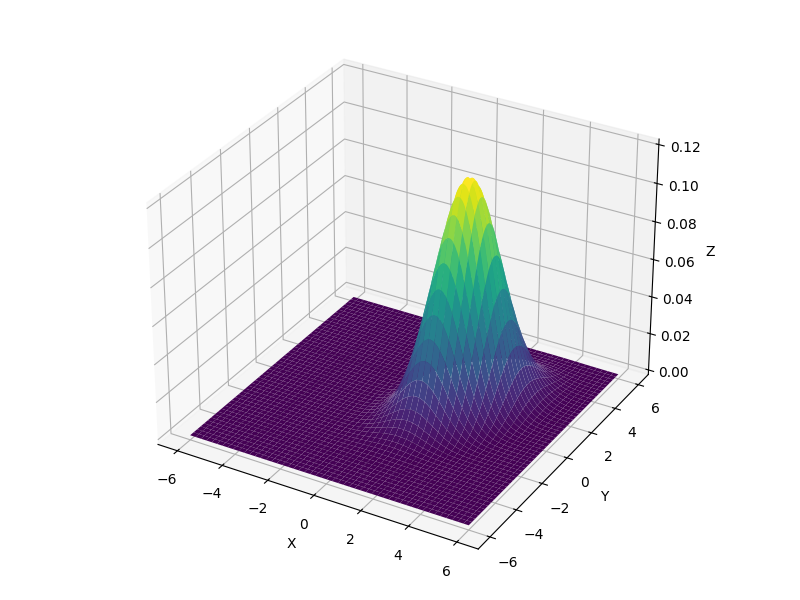
\includegraphics[width=0.7\textwidth]{./pdf-1.png}

\boldmath
\subsection{Plot the joint pdf with given values in a, if $y=\mu_y=1$}
\unboldmath

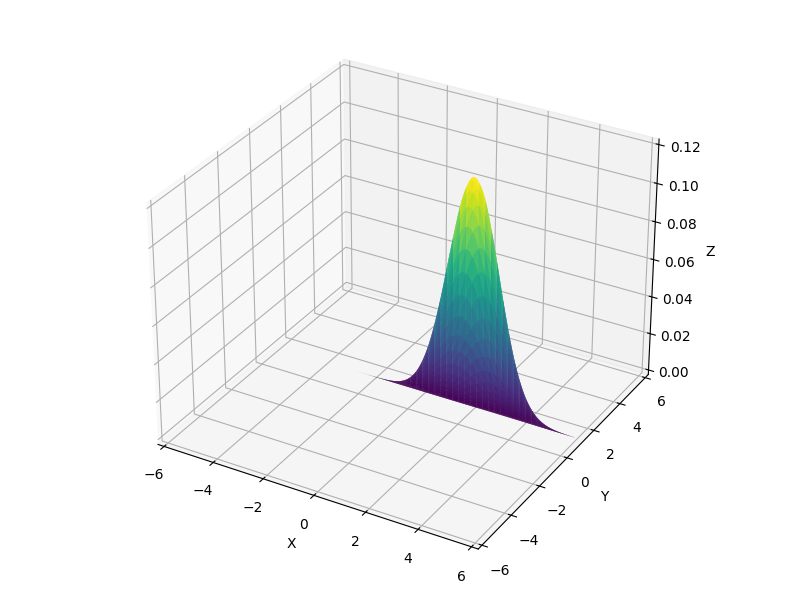
\includegraphics[width=0.7\textwidth]{./pdf-2.png}

\boldmath
\subsection{Plot the joint pdf with given values in a, if $x=\mu_x=2$}
\unboldmath

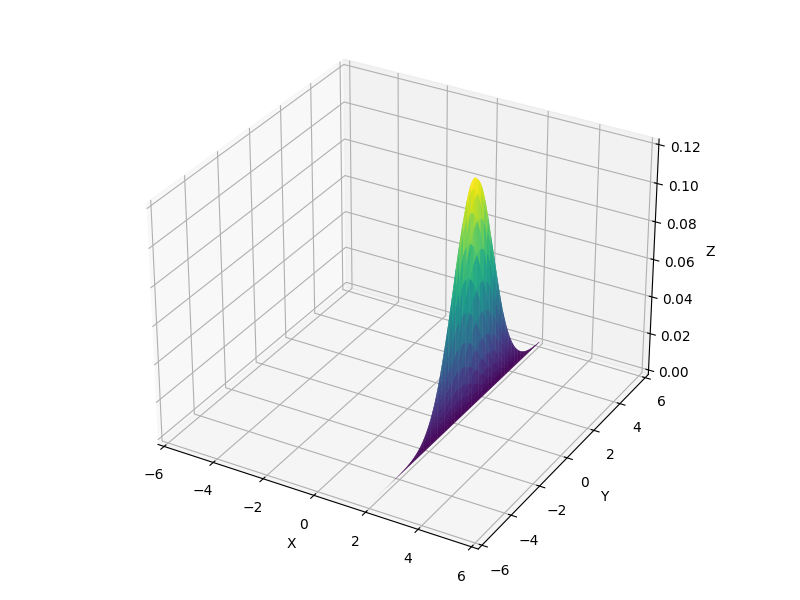
\includegraphics[width=0.7\textwidth]{./pdf-3.png}

\section{Conclusion}

In conclusion, this project has demonstrated the utility of joint Gaussian probability
density functions (PDFs) in understanding the interdependencies between variables.
By visualizing the PDFs and examining slices at constant values, we've been able to
examine the distribution's behavior. \\ \\
The observation that fixing one variable results in a slice of the original distribution
highlights the correlation and interdependency between variables. This understanding
is crucial for making informed decisions in scientific and engineering disciplines. \\ \\
Overall, this project emphasizes the importance of probability theory and statistical
analysis in characterizing complex systems, providing a solid foundation for future
content in the course.

\end{document}
